\documentclass[a4paper,12pt]{article}
\usepackage{graphicx}
\usepackage{fancyhdr}
\usepackage{xcolor}
\usepackage{hyperref}
\usepackage{amsmath,amssymb}
\usepackage{enumitem}
\usepackage{makecell}
\usepackage{textcomp}
\usepackage{listings}
\usepackage{cite}
\usepackage{caption}

\begin{document}

% ---------- Custom Header: ONLY ON FIRST PAGE ----------
\fancypagestyle{firstpage}{
\fancyhf{}
\fancyhead[L]{
    \includegraphics[width=8cm, height=1.7cm]{IIITB-COMET-Logo.png}
}
\fancyhead[R]{
    Project Title: Voice Based with UGV Obstacles Detection Model \\
    Name: Ajay Krishna DM \\
    Guide: Srikanth Reddy \\
    Batch: COMETFWC037 \\
    Date: 22 October 2025
}
\renewcommand{\headrulewidth}{0pt}
\fancyfoot[C]{\thepage}
}
\thispagestyle{firstpage}
% -------------------------------------------------------

\vspace*{1cm}
\begin{center}
    {\LARGE \textbf{\textcolor{blue}{Voice Based UGV Control with Obstacle Detection}}}
\end{center}

\section*{Abstract}
In this paper, we demonstrate how to guide an unmanned ground vehicle (UGV) using a gamepad interface as well as voice commands. This is done through an android application for sensing voice or touch on the phone and relaying the control data to the UGV via Bluetooth. An ultrasonic sensor is used to detect and avoid obstacles automatically. This platform offers a low-cost alternative for implementing artificial intelligence (AI) algorithms on embedded hardware.

\section{Introduction}
Autonomous navigation has been a major area of research in robotics, with pioneering projects such as 
\cite{thrun2006stanley}, 
\cite{urmson2008boss, montemerlo2008junior}, demonstrating autonomous navigation in complex environments. 
End-to-end learning approaches, such as NVIDIA's system for self-driving cars \cite{bojarski2016end}, have further simplified navigation pipelines by mapping sensor inputs directly to control outputs. 
Speech-based human-robot interaction has enabled intuitive control of robots, including intelligent wheelchairs and mobile robots \cite{li2017speech, prasad2013voice, vasudevan2010speech}, while datasets such as Google’s Speech Commands \cite{warden2018speech} have accelerated the development of voice-controlled systems. 

Inspired by the above, this work presents a prototype using an ESP32 microcontroller, L293D motor driver, and an ultrasonic sensor to build a voice-enabled toy car that can detect obstacles while being controlled through voice and Bluetooth.

\section{Hardware Setup}
The components used in this project and their description are listed in Table \ref{table:list}.
\begin{table}[!h]
  \centering
  \begin{tabular}{|c|c|}
  \hline
  \textbf{Component} & \textbf{Description} \\
  \hline
  ESP32 & Microcontroller with Bluetooth and Wi-Fi \\
  L293D & Motor Driver IC \\
  Ultrasonic Sensor (HC-SR04) & Measures distance to detect obstacles \\
  DC Motors & Drive the toy car wheels \\
  Chassis & Car body to hold components \\
  Power Bank & Power source for ESP32 \\
  Jumper Wires & For connections \\
  \hline
  \end{tabular}
  \caption{List of Components}
  \label{table:list}
\end{table}

\subsection*{Assembly Steps}
\begin{enumerate}
\item Assemble the chassis, fix the motors, and mount the wheels.
\item Fix the breadboard on the base of the car.
\item Plug the \textbf{L293D} motor driver IC on the breadboard.
\item Connect L293D output pins to the motors ($M_1, M_2$).
\item Connect ESP32 to L293D as per motor control pins.
\item Connect the ultrasonic sensor to the ESP32 as shown in Table \ref{table:ultrasonic}.
\end{enumerate}

\begin{table}[!h]
  \centering
  \begin{tabular}{|c|c|}
  \hline
  \textbf{Ultrasonic Pin} & \textbf{ESP32 Pin} \\
  \hline
  VCC & 5V \\
  GND & GND \\
  TRIG & GPIO 5 \\
  ECHO & GPIO 18 \\
  \hline
  \end{tabular}
  \caption{Ultrasonic Sensor and ESP32 Connections}
  \label{table:ultrasonic}
\end{table}

% ---------------- Added Images ----------------
\subsection*{Dabble App Interface}
\begin{figure}[!h]
\centering
\includegraphics[width=0.6\textwidth]{dabble_home.jpg}
\caption{Dabble App Main Interface}
\end{figure}

\subsection*{L293D Motor Driver IC}
\begin{figure}[!h]
\centering
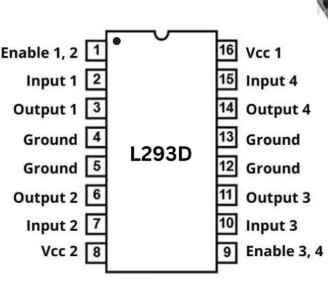
\includegraphics[width=0.5\textwidth]{L293D_IC.png}
\caption{Pin Diagram of L293D Motor Driver IC}
\end{figure}

\subsection*{ESP32 Microcontroller Board}
\begin{figure}[!h]
\centering
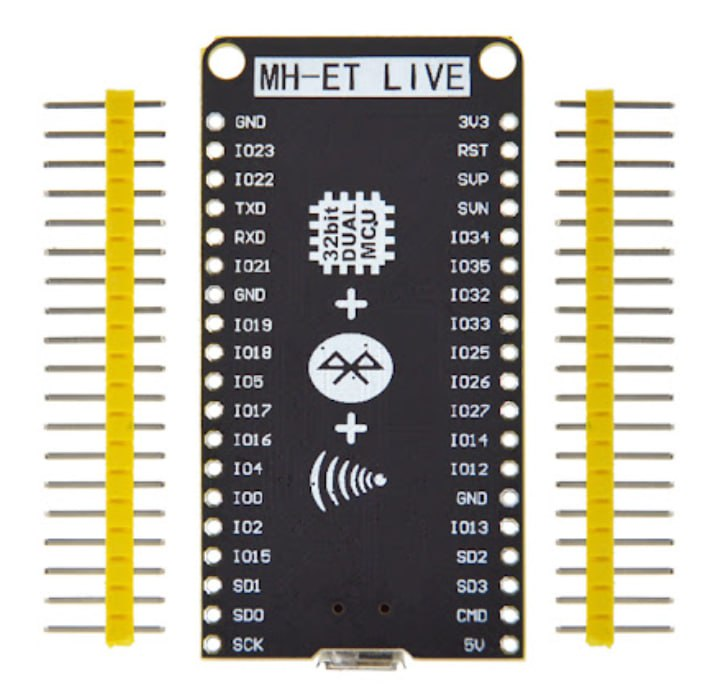
\includegraphics[width=0.6\textwidth]{ESP32.png}
\caption{ESP32 MH-ET LIVE Board}
\end{figure}

\begin{figure}[!h]
\centering
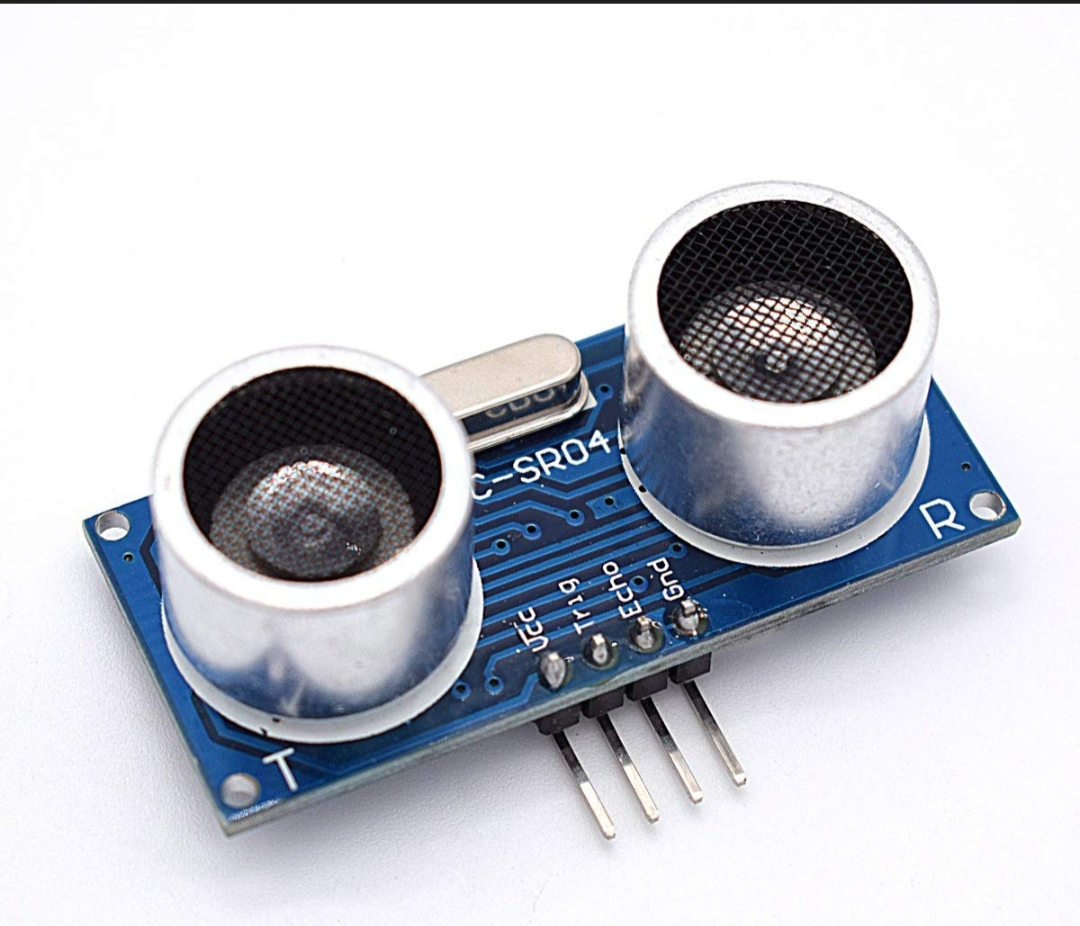
\includegraphics[width=0.6\textwidth]{ultrasonic_sensor.jpg}
\caption{HC-SR04 Ultrasonic Sensor}
\label{fig:ultrasonic}
\end{figure}

\section{Software Setup}

\subsection{Dabble App Control}
\begin{enumerate}
\item Install the {\em Dabble} app from the Google Play Store.
\item Upload code to ESP32 using PlatformIO from the following link:
\fbox{\parbox{\linewidth}{%
\url{https://github.com/gadepall/voice-ugv/blob/main/codes/dabble_gamepad.cpp}%
}}
\item Replace contents of \texttt{src/main.cpp} in PlatformIO with the above code and upload.
\item Connect the ESP32 to the phone via Bluetooth.
\item Use the Gamepad in the Dabble app to control directions — Forward, Back, Left, Right.
\end{enumerate}

\subsection{Voice Control using Arduino Bluetooth Controller}
\begin{enumerate}
\item Install the {\em Arduino Bluetooth Controller} app.
\item Upload the voice control code to ESP32 using PlatformIO:
\fbox{\parbox{\linewidth}{%
\url{https://github.com/gadepall/voice-ugv/blob/main/codes/ABC_voice.cpp}%
}}
\item Connect via Bluetooth and select the “Voice Control” mode.
\item Use commands: \textit{Left, Right, Forward, Back, Stop}.
\end{enumerate}

\subsection{Obstacle Detection with Ultrasonic Sensor}
The ultrasonic sensor detects obstacles by emitting sound waves and measuring the time it takes for the echo to return.  
If the distance is below a threshold (e.g., 20 cm), the ESP32 automatically stops or diverts the car to avoid collision.

\begin{lstlisting}[language=C++, caption=Sample Ultrasonic Code Snippet]
#define TRIG 5
#define ECHO 18

void loop() {
  long duration;
  int distance;
  digitalWrite(TRIG, LOW);
  delayMicroseconds(2);
  digitalWrite(TRIG, HIGH);
  delayMicroseconds(10);
  digitalWrite(TRIG, LOW);
  duration = pulseIn(ECHO, HIGH);
  distance = duration * 0.034 / 2;

  if (distance < 20) {
    stopCar(); // Stop motors
  } else {
    moveForward();
  }
}
\end{lstlisting}

\section{Conclusion and Future Work}
We have successfully built a voice-controlled UGV equipped with an ultrasonic sensor for obstacle detection. This system demonstrates an efficient low-cost model for AI-based control and interaction. Future improvements include integrating onboard speech recognition and path-planning algorithms directly on the ESP32 to eliminate the need for external servers.

\bibliographystyle{plain}
\bibliography{references}

\end{document}
